%% This is file `elsarticle-template-1-num.tex',
%%
%% Copyright 2009 Elsevier Ltd
%%
%% This file is part of the 'Elsarticle Bundle'.
%% ---------------------------------------------
%%
%% It may be distributed under the conditions of the LaTeX Project Public
%% License, either version 1.2 of this license or (at your option) any
%% later version.  The latest version of this license is in
%%    http://www.latex-project.org/lppl.txt
%% and version 1.2 or later is part of all distributions of LaTeX
%% version 1999/12/01 or later.
%%
%% Template article for Elsevier's document class `elsarticle'
%% with numbered style bibliographic references
%%
%% $Id: elsarticle-template-1-num.tex 149 2009-10-08 05:01:15Z rishi $
%% $URL: http://lenova.river-valley.com/svn/elsbst/trunk/elsarticle-template-1-num.tex $
%%
\documentclass[preprint,12pt]{elsarticle}

\usepackage[colorlinks]{hyperref}
\usepackage[colorinlistoftodos]{todonotes}
\usepackage{verbatim}

%% Use the option review to obtain double line spacing
%% \documentclass[preprint,review,12pt]{elsarticle}

%% Use the options 1p,twocolumn; 3p; 3p,twocolumn; 5p; or 5p,twocolumn
%% for a journal layout:
%% \documentclass[final,1p,times]{elsarticle}
%% \documentclass[final,1p,times,twocolumn]{elsarticle}
%% \documentclass[final,3p,times]{elsarticle}
%% \documentclass[final,3p,times,twocolumn]{elsarticle}
%% \documentclass[final,5p,times]{elsarticle}
%% \documentclass[final,5p,times,twocolumn]{elsarticle}

%% The graphicx package provides the includegraphics command.
\usepackage{graphicx}
%% The amssymb package provides various useful mathematical symbols
\usepackage{amssymb}
%% The amsthm package provides extended theorem environments
%% \usepackage{amsthm}

%% The lineno packages adds line numbers. Start line numbering with
%% \begin{linenumbers}, end it with \end{linenumbers}. Or switch it on
%% for the whole article with \linenumbers after \end{frontmatter}.
\usepackage{lineno}

%% natbib.sty is loaded by default. However, natbib options can be
%% provided with \biboptions{...} command. Following options are
%% valid:

%%   round  -  round parentheses are used (default)
%%   square -  square brackets are used   [option]
%%   curly  -  curly braces are used      {option}
%%   angle  -  angle brackets are used    <option>
%%   semicolon  -  multiple citations separated by semi-colon
%%   colon  - same as semicolon, an earlier confusion
%%   comma  -  separated by comma
%%   numbers-  selects numerical citations
%%   super  -  numerical citations as superscripts
%%   sort   -  sorts multiple citations according to order in ref. list
%%   sort&compress   -  like sort, but also compresses numerical citations
%%   compress - compresses without sorting
%%
%% \biboptions{comma,round}

% \biboptions{}

\journal{DAACH}

\begin{document}

\begin{frontmatter}

%% Title, authors and addresses

\title{Asymmetry of Caddo Ceramics from the Washington Square Mound Site: An Exploratory Analysis}

%% use the tnoteref command within \title for footnotes;
%% use the tnotetext command for the associated footnote;
%% use the fnref command within \author or \address for footnotes;
%% use the fntext command for the associated footnote;
%% use the corref command within \author for corresponding author footnotes;
%% use the cortext command for the associated footnote;
%% use the ead command for the email address,
%% and the form \ead[url] for the home page:
%%
%% \title{Title\tnoteref{label1}}
%% \tnotetext[label1]{}
%% \author{Name\corref{cor1}\fnref{label2}}
%% \ead{email address}
%% \ead[url]{home page}
%% \fntext[label2]{}
%% \cortext[cor1]{}
%% \address{Address\fnref{label3}}
%% \fntext[label3]{}


%% use optional labels to link authors explicitly to addresses:
%% \author[label1,label2]{<author name>}
%% \address[label1]{<address>}
%% \address[label2]{<address>}

\author[1]{Robert Z. Selden Jr. \corref{cor1}}

\address[1]{Center for Regional Heritage Research, Stephen F. Austin State University, Nacogdoches, USA}

\cortext[cor1]{Corresponding author, Robert Z. Selden Jr. (seldenjrz@sfasu.edu)}

\begin{abstract}
%% Text of abstract
While pursuing a study of 3D geometric morphometrics for ceramic burial vessels that often articulate with the Native American Graves Protection and Repatriation Act (NAGPRA) from the ancestral Caddo region, there have been no shortage of potentially meaningful observations, one of which--rotational asymmetry in coil-built vessels--is discussed here. Using Geomagic Design X (reverse-engineering software) and Geomagic Control X (inspection software), metrics associated with rotational asymmetry were generated then analyzed. Results indicate variable asymmetry among the different vessel shapes (i.e., bottles, jars, etc.), which may augment and strengthen studies and discussion of vessel form. Future directions include the incorporation of directional and--possibly--fluctuating asymmetry measures for the widest vessel profiles. Preliminary results point toward substantive analytical gains that can be used to augment more traditional ceramic analyses as well as geometric morphometric studies of ceramic vessel shape. 
\end{abstract}

\begin{keyword}
3D \sep  Symmetry \sep Asymmetry \sep Geometric Morphometrics \sep Ceramics 
%% keywords here, in the form: keyword \sep keyword

%% MSC codes here, in the form: \MSC code \sep code
%% or \MSC[2008] code \sep code (2000 is the default)

\end{keyword}

\end{frontmatter}

%%
%% Start line numbering here if you want
%%
\linenumbers

%% main text
\section{Introduction}
\label{S:1}

The Caddo peoples inhabited areas of what are today Arkansas, Louisiana, Oklahoma, and Texas from ca. A.D. 800/850-1838 \citep{Perttula:2}. They were horticulturalists as well as agriculturalists, with a particular focus on maize cultivation \citep{Perttula:2, Perttula:3, Wilson:1}. Their ancestral predecessors were various Woodland period communities that developed between ca. 500 B.C. and A.D. 800 \citep{Selden:8}. Caddo communities and separate population groups may have first emerged within two areas: the Great Bend of the Red River in southwestern Arkansas and northwest Louisiana, and in the Arkansas River basin in eastern Oklahoma \citep{Story:1}. However, other important communities developed early on in East Texas and in the Ouachita River basin in southwest Arkansas \citep{Story:1}. Those ceramics employed within the framework of this analysis are from the Washington Square Mound site (41NA49), a Middle Caddo (ca. A. D. 1200-1450) mound site located in Nacogdoches, Texas (Figure ~\ref{fig:Figure 1}).

\begin{figure}[ht]\centering
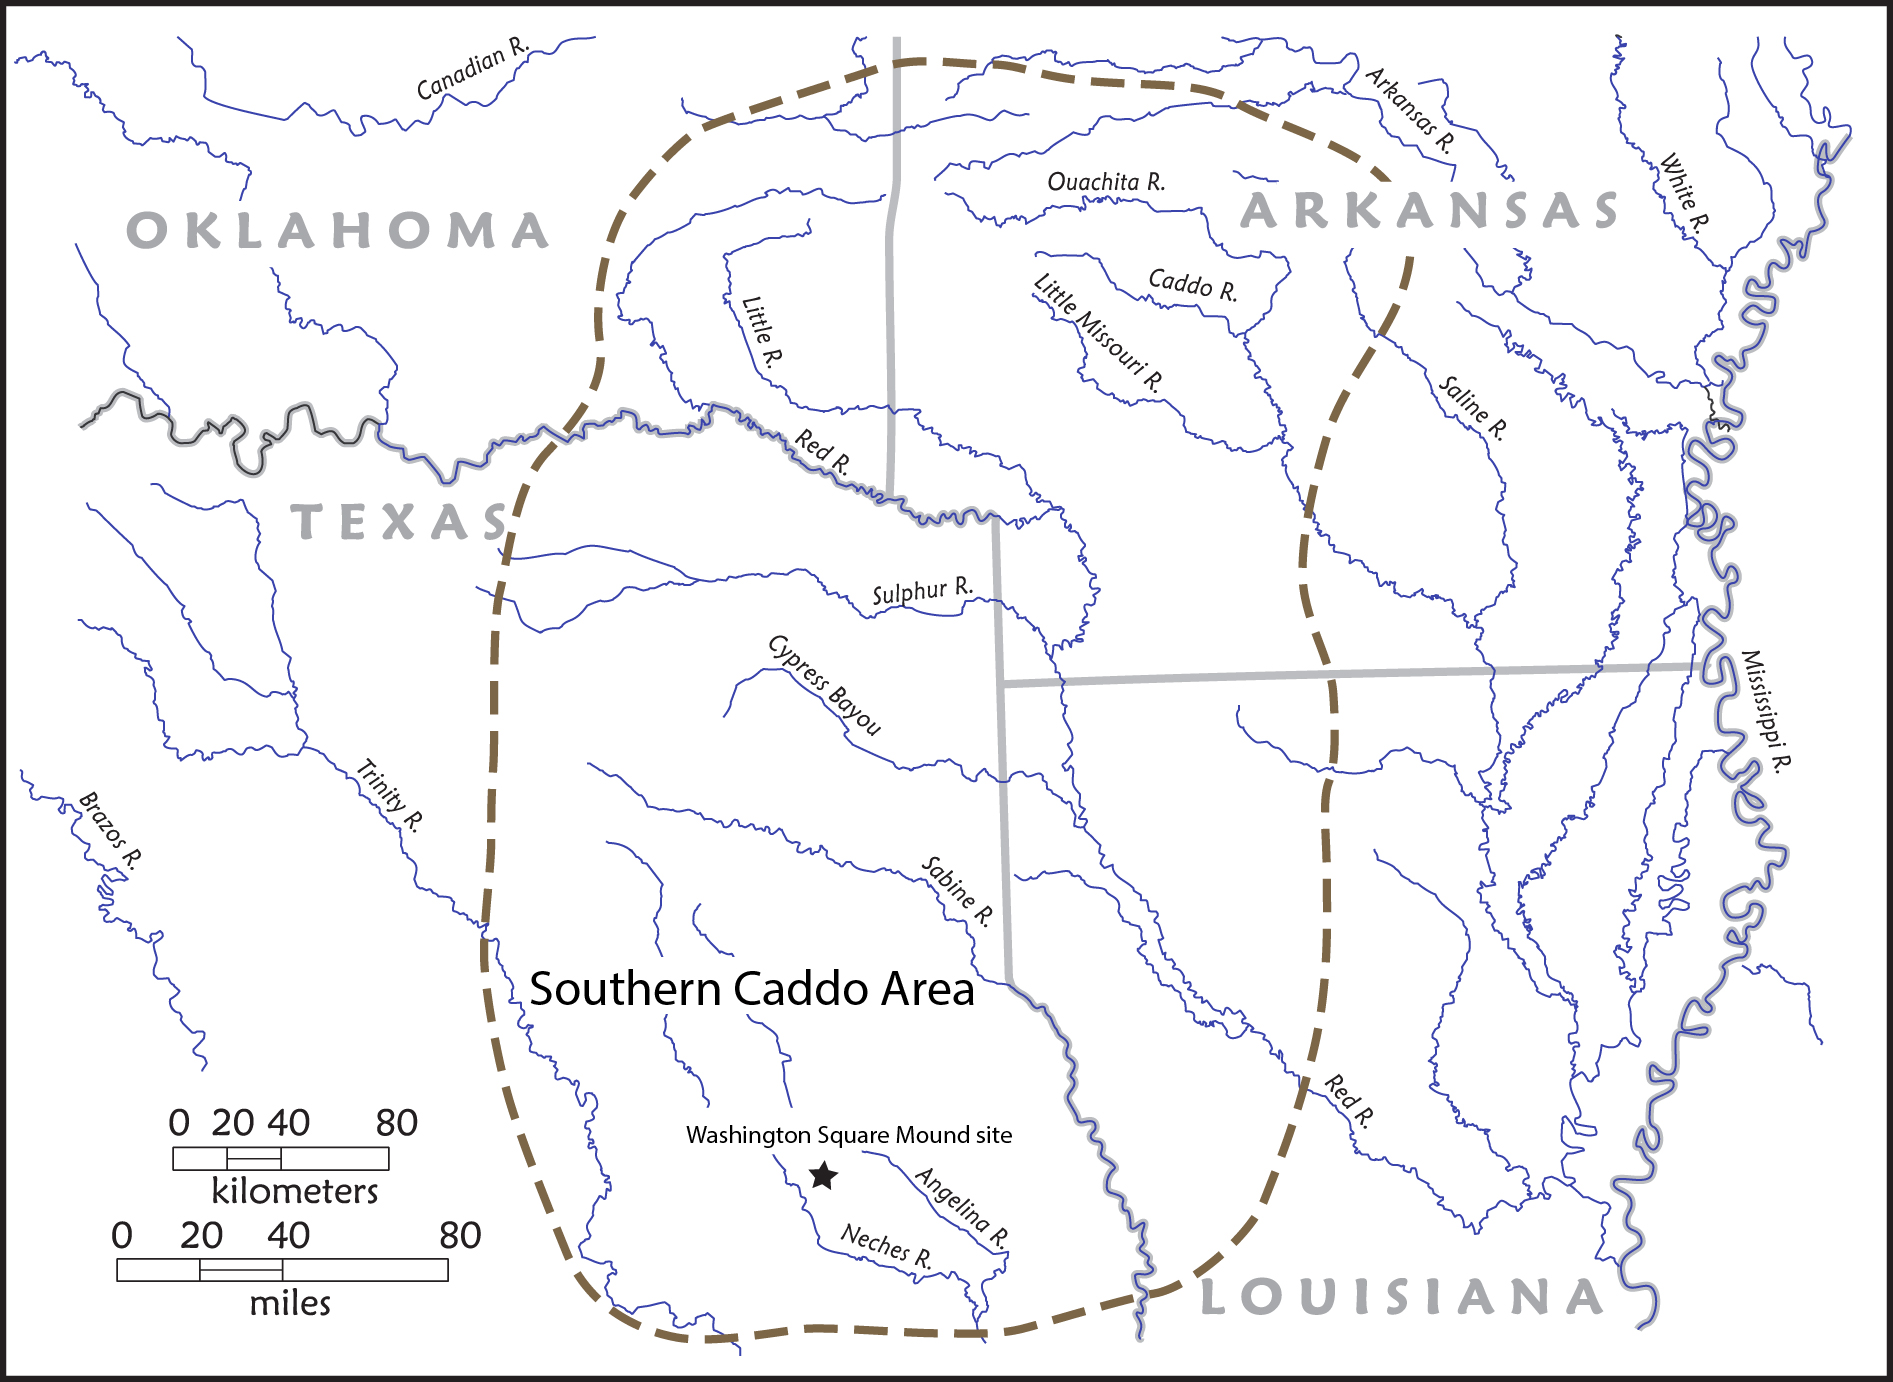
\includegraphics[width=\linewidth]{SS_2015_Figure_1}
\caption{The Southern Caddo Area and the Washington Square Mound site.}
\label{fig:Figure 1}
\end{figure}

While elements of Caddo life share many similarities with (U.S.) Southeastern Mississippian cultures, cultural developments in the Caddo area do not appear to have developed in concert with their Mississippian counterparts \citep{Blitz:1, Livingood:1}. This has led archaeologists to consider Caddo developments as an expression of local and regional processes linked culturally and temporally to preceding Woodland period groups and to interactions between different Caddo groups \citep{Perttula:4, Perttula:2}. Caddo trade networks extended from Cahokia in the north \citep{Smith:1, Foster:1}, to the Pueblo villages of New Mexico in the west \citep{Smith:1}, to the Acansa and Taensa Indians on the Mississippi and Arkansas rivers to the east \citep{Foster:1}. Manufacturers of such sought-after items as bows constructed of Osage orange (Bois d`arc), decorated fine ware pottery, salt, and food products, the Caddo were well situated within local and extended trade networks \citep{LaVere:1, Perttula:5, Smith:1, Swanton:1}.

\subsection{Asymmetry}

Coil-built ceramics (like those of the Caddo) are abundant in the archaeological record of the Americas, and are primarily segregated and assigned to specific temporal and spatial components based upon surficial attributes and decorative motifs. The lack of a substantive discourse among ceramic analysts regarding issues of vessel shape and asymmetry can likely be linked to the perceived inability to fully characterize the enormous scope of variation that occurs throughout ceramic assemblages, coupled with the fact that the majority of analysts primarily work with sherd assemblages more regularly than with whole vessels. Adding to this are the tight timelines associated with cultural resource management (CRM) analyses, the expense and time commitment associated with collecting and analyzing 3D data, navigating burial legislation (NAGPRA, etc.), highly variable bureaucratic semantics, and the oft-burdensome museum or repository bureaucracy involved with accessing and digitizing collections for use as a comparative resource. For these and many other reasons, it quickly becomes apparent why such a deficit of knowledge remains for these data rich--yet understudied--cultural resources. 

Recent forays into the symmetry and asymmetry related to ceramic artifacts are more regularly focused upon decorative elements \citep{Pluckhahn:1} than issues of vessel shape or form \citep{Girrulat:1}. It is within a study of the latter where the various components of this effort begin to take shape \citep{Hodgson:1}, raising potentially significant questions regarding the ceramic technological organization of the Caddo people. Using the results of this analysis, differences in Caddo fine wares and utility wares could be compared to explore whether a ceramic vessel with a lower deviation from rotational symmetry might have been seen as more attractive, which may provide further insight into the value of specific elements of the Caddo ceramic economy. Measures of symmetry and asymmetry are also compared between the variable categories of vessel shape (bowl, bottle, etc.) to investigate whether, and what manner of, variation may exist among them. Further still, these metrics might help to clarify additional patterns that are becoming more apparent in studies of geometric morphometrics for ceramic artifacts \citep{Selden:2}.

\subsection{Research Potential} 

The degree to which this approach might better demarcate between elements of elite and commoner production strategies \citep{Inomata:1} remains unknown; however, it may be possible to leverage morphological components from ceramics with known cultural associations (i.e., elite, commoner, etc.) to elaborate upon differential production strategies and manufacturing processes \citep{Wang:1}. For instance, should a higher degree of symmetry be found to correlate with elite burials or ceremonial contexts, and not with those contexts associated with Caddo commoners, arguments for the attractiveness of symmetry \cite{Little:1, Little:2, Little:3} and shape \cite{Shott:2, Shott:3, Shott:4, Slice:1} for specific elements of these vessels might be more gainfully argued in concert with the associated qualitative attributes. The notion of attractiveness in this context could help us to better couch our ideas related to the Caddo ceramic economy.

While exploratory, this approach may also yield additional insight into whether it is possible to discriminate between basic vessel forms (i.e., bowl, bottle, jar, etc.) using attributes associated with rotational asymmetry. Results from the analyses of rotational asymmetry are discussed herein, and future directions posited that include using landmarks and semi-landmarks from the geometric morphometric analysis to incorporate analyses of directional and fluctuating asymmetry. Results of these analyses are then added to those data from a previous documentation effort. Outcomes of the analysis have implications for the organization of craft production \citep{Costin:2}, to include explanations of technological varieties, which inform upon basic tenets of the local economy \citep{Costin:1}. This method may also prove fruitful in addressing variable asymmetry between coil- and wheel-built vessels, helping to further refine our ideas associated with variable ceramic manufacturing practices and processes \citep{Sinopoli:1}.

\section{Methods}

The three-dimensional (3D) scan data used in this analysis were collected using a ZScanner 700CX running VXelements software via the scanner direct control feature in Geomagic Design X, and all data are open access and available for download on Zenodo \cite{selden:19, Selden:18, Selden:17, Selden:16, Selden:15, Selden:14, Selden:13, Selden:12, Selden:11, Selden:10}. The use of Geomagic Design X in this research program streamlines the 3D scanning process by allowing analysts to scan, post-process, and generate reference geometry—-and in this case also a rotationally symmetrical surface, landmarks, and sliding adaptive semilandmark data points—-in a single interface \cite{Selden:20}. 

\subsection{Missing Data}

As research efforts aimed at the development and integration of geometric morphometrics for Caddo ceramics continues, peripheral (unexpected) analytical insights are beginning to arise on a more regular basis. As those methods associated with the analyses have matured \citep{Selden:2}, the number of 3D meshes suitable for analysis initially declined. This occurred in part to a necessary developmental phase within the larger research design, where every nearly-intact vessel was scanned. That practice resulted in the collection of 3D meshes that can continue to be used to test and improve upon  methods associated with these analyses. As the analysis of each collection draws to a close, methods continue to be revised to align with iterative improvements in the evolution of the methodological approach. Initially, the landmarks (LM) and semilandmarks (sLM) used in the analysis were applied a manner that actively avoided areas of missing data \citep{Selden:2}; however, in the pursuit of a more standardized and replicable approach, many vessels from the initial analysis could no longer be used due to the overlap of splines with an area of missing data. 

The integration of Geomagic Design X and Geomagic Control X in this research design has greatly streamlined the analytical process. Using this software, we can scan directly into the same platform used to post-process the meshes and populate reference geometry, then populate LM and sLM data for the geometric morphometric analyses. Other similar software packages exist (PolyWorks, etc.), and while this approach is focused only upon Geomagic Design X and Control X, similar approaches could be employed using those programs as well. Once processed, it is important to outline how mesh defects and missing data were addressed for each scan (keeping in mind that each is unique).

\subsubsection{Methods used to Address Missing Data} 

When the scanning process is complete, the file is opened in Geomagic Design X where the processing of those files begins. In general, two kinds of missing data are regularly encountered with 3D scanning practices; one where those data are genuinely missing from the original model; the other where those data were not collected by the scanner. It is important to identify which relates most readily with those data missing from each scan. This information can be used to help identify regions of certain artifact forms that require more attention during the scanning process, perhaps due to areas of high reflectivity or other known (and quickly remedied) issues. If those data missing from the mesh are present on the artifact, it is best to begin with scanning that particular piece a second time. Those data can then be merged with data from the first scan, beginning post-processing by using the best possible scan with the fewest missing data. 

Prior to addressing missing data, each scan is processed using the Healing Wizard function. The Healing Wizard function runs a variety of checks for non-manifold poly-vertices, folded poly-faces, dangling poly-faces, small clusters, small poly-faces, non-manifold poly-faces, crossing poly-faces, and small tunnels for each scan. This step corrects abnormalities in each mesh, decreasing the chance of encountering an error while addressing areas of missing data.

To align each scan, a reference vector (revolving axis) was inserted, followed by a reference point at the confluence of the vector and the mesh at the central base (projection). Region groups were then used to define the basal plane. All three elements (vector, point and plane) of reference geometry were utilized in an interactive alignment, with the reference plane as the moving plane, the reference vector as the moving vector, and the reference point as the moving point. Alignment has proven to be an important factor in downstream analyses (and landmark/semilandmark application), particularly when making the transition from Geomagic Design X and Control X to SolidWorks or other CAD-based software. 

Due to the variable nature of the archaeological record, some ceramics are well-preserved while others fragment, weather and decompose at fluctuating (often much quicker) rates, depending upon a wide range of factors. The bulk of Caddo ceramic vessels scanned for the geometric morphometrics project are comprised of this latter group, and were--most often--reassembled by the repository or curation facility. 

\subsubsection{Addressing Areas with Missing Data}

The splines used in the geometric morphometric analysis dictate the location(s) of missing data that must be addressed prior to populating LM/sLM data. Each situation requires a unique solution, and each has the capacity to impact the analysis. In an effort to select the method that deviates least from the original surface geometry, an area adjacent to the hole is cut out and deleted to create another hole of similar size. A Caddo NAGPRA vessel from the Turner Collection with an area of missing data will be used to illustrate this approach.

To begin, the aligned mesh is exported as an ASCII.stl that will be used as the control. A hole is then cut in the existing mesh adjacent to the missing data. The mesh is saved as an ASCII.stl, and will be imported and patched using each of the three functions (defeature, edit boundaries, and fill holes), then each mesh is saved as a unique ASCII.stl. Since the control model was aligned prior to exporting the mesh with the hole, that alignment carries over to each of the resultant meshes (control, hole, defeature, edit boundaries, and fill holes). Once complete, those meshes produced by each of the three hole-filling functions are compared against the control in Geomagic Control X.

Geomagic Control X is inspection software traditionally used to compare 3D CAD models against meshes to identify areas of wear on machined parts. In this case, the nominal data (control) is contrast against each of the three hole-filling functions (scan data) to identify which deviates least from the original mesh (Figure ~\ref{fig:Figure 4}). These results guide the decision-making strategy with regard to the post-processing procedure for areas of missing data, allowing modelers to make more informed decisions about which function to use.

\begin{figure}[ht]\centering
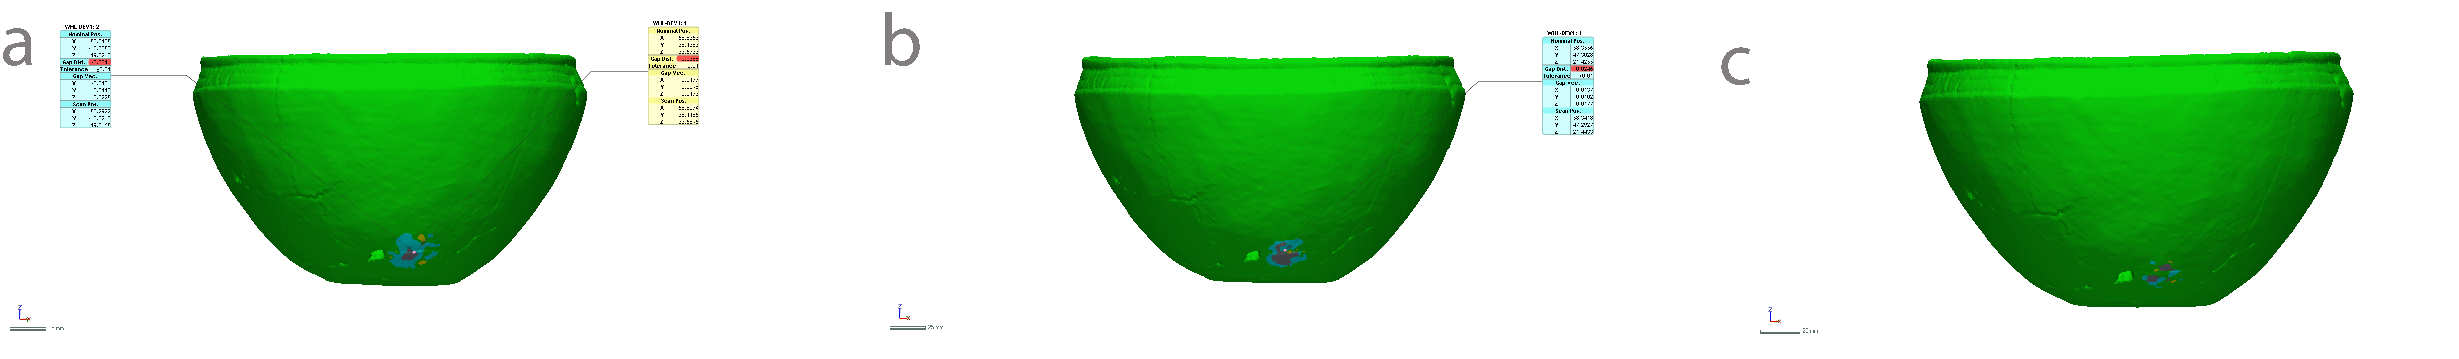
\includegraphics[width=\linewidth]{FigMData}
\caption{Control data contrast with (a) defeature, (b) edit boundaries and (c) fill holes.}
\label{fig:Figure 4}
\end{figure}

In this particular case, the fill holes feature deviates least from the original 3D mesh. Call-outs were only issued for those deviations over 0.02mm, and in this instance, the maximum deviation from the control data was 0.0184mm using the fill holes function. Prior to employing the fill holes function as the remedy for this area of missing data, a clean cut was made in the mesh around the hole and a second pass of the healing wizard was used to correct for any errors created by the cut. The final mesh was then ready for use in the analysis.

Among those lessons learned throughout this process is a subjective triage system that dictates which vessels get scanned, and which do not. In short, some areas of missing data cannot be remedied while maintaining a high degree of confidence regarding the resultant geometry. While the three functions discussed here are ample to address the bulk of our concerns involving how we might best approach missing data in these smaller areas, more robust methods are warranted for larger holes, for which processing time increases exponentially. 

In the sample of scan data collected for the 3D geometric morphometrics study, around 15 percent are unable to be used due to the location of a large (often around 50mm and larger) missing sherd. Certainly methods exist to address the majority of missing data in those meshes; however, these are not included in the study of geometric morphometrics. Instead, those meshes are used to document design-based elements and motifs \citep{Selden:2}.

\subsection{Quantifying Deviation from Rotational Symmetry}

Using 10 3D scans of Caddo burial (NAGPRA) vessels from the Washington Square Mound site (41NA49) in Nacogdoches, Texas, a method was devised to assess the deviation of coil-built ceramics from a rotationally symmetrical surface. For this analysis, a unique surface was generated for each of the Caddo vessels in the sample (Figure ~\ref{fig:Figure 5}). To create the symmetrical surface, the widest point of each vessel was identified while each vessel was oriented along the basal plane. For the purpose of this research design, this same point was then used in the geometric morphometric analysis. This approach provided those data needed to revolve the widest profile 360-degrees around the vector (central axis). To identify the widest point of the vessel, a mesh sketch was created using the reference point as the central point of a circle. The sketch (circle) was extruded in both directions to create a surface that covered the vessel completely, and deviations between the surface and mesh were calculated to identify the widest point of the vessel. A reference plane was then inserted along the widest profile, coplanar to the central vector. That plane was then used as the basis for a second mesh sketch of the widest profile, which was subsequently revolved around the central axis to create each rotationally-symmetrical surface.

\begin{figure}[ht]\centering
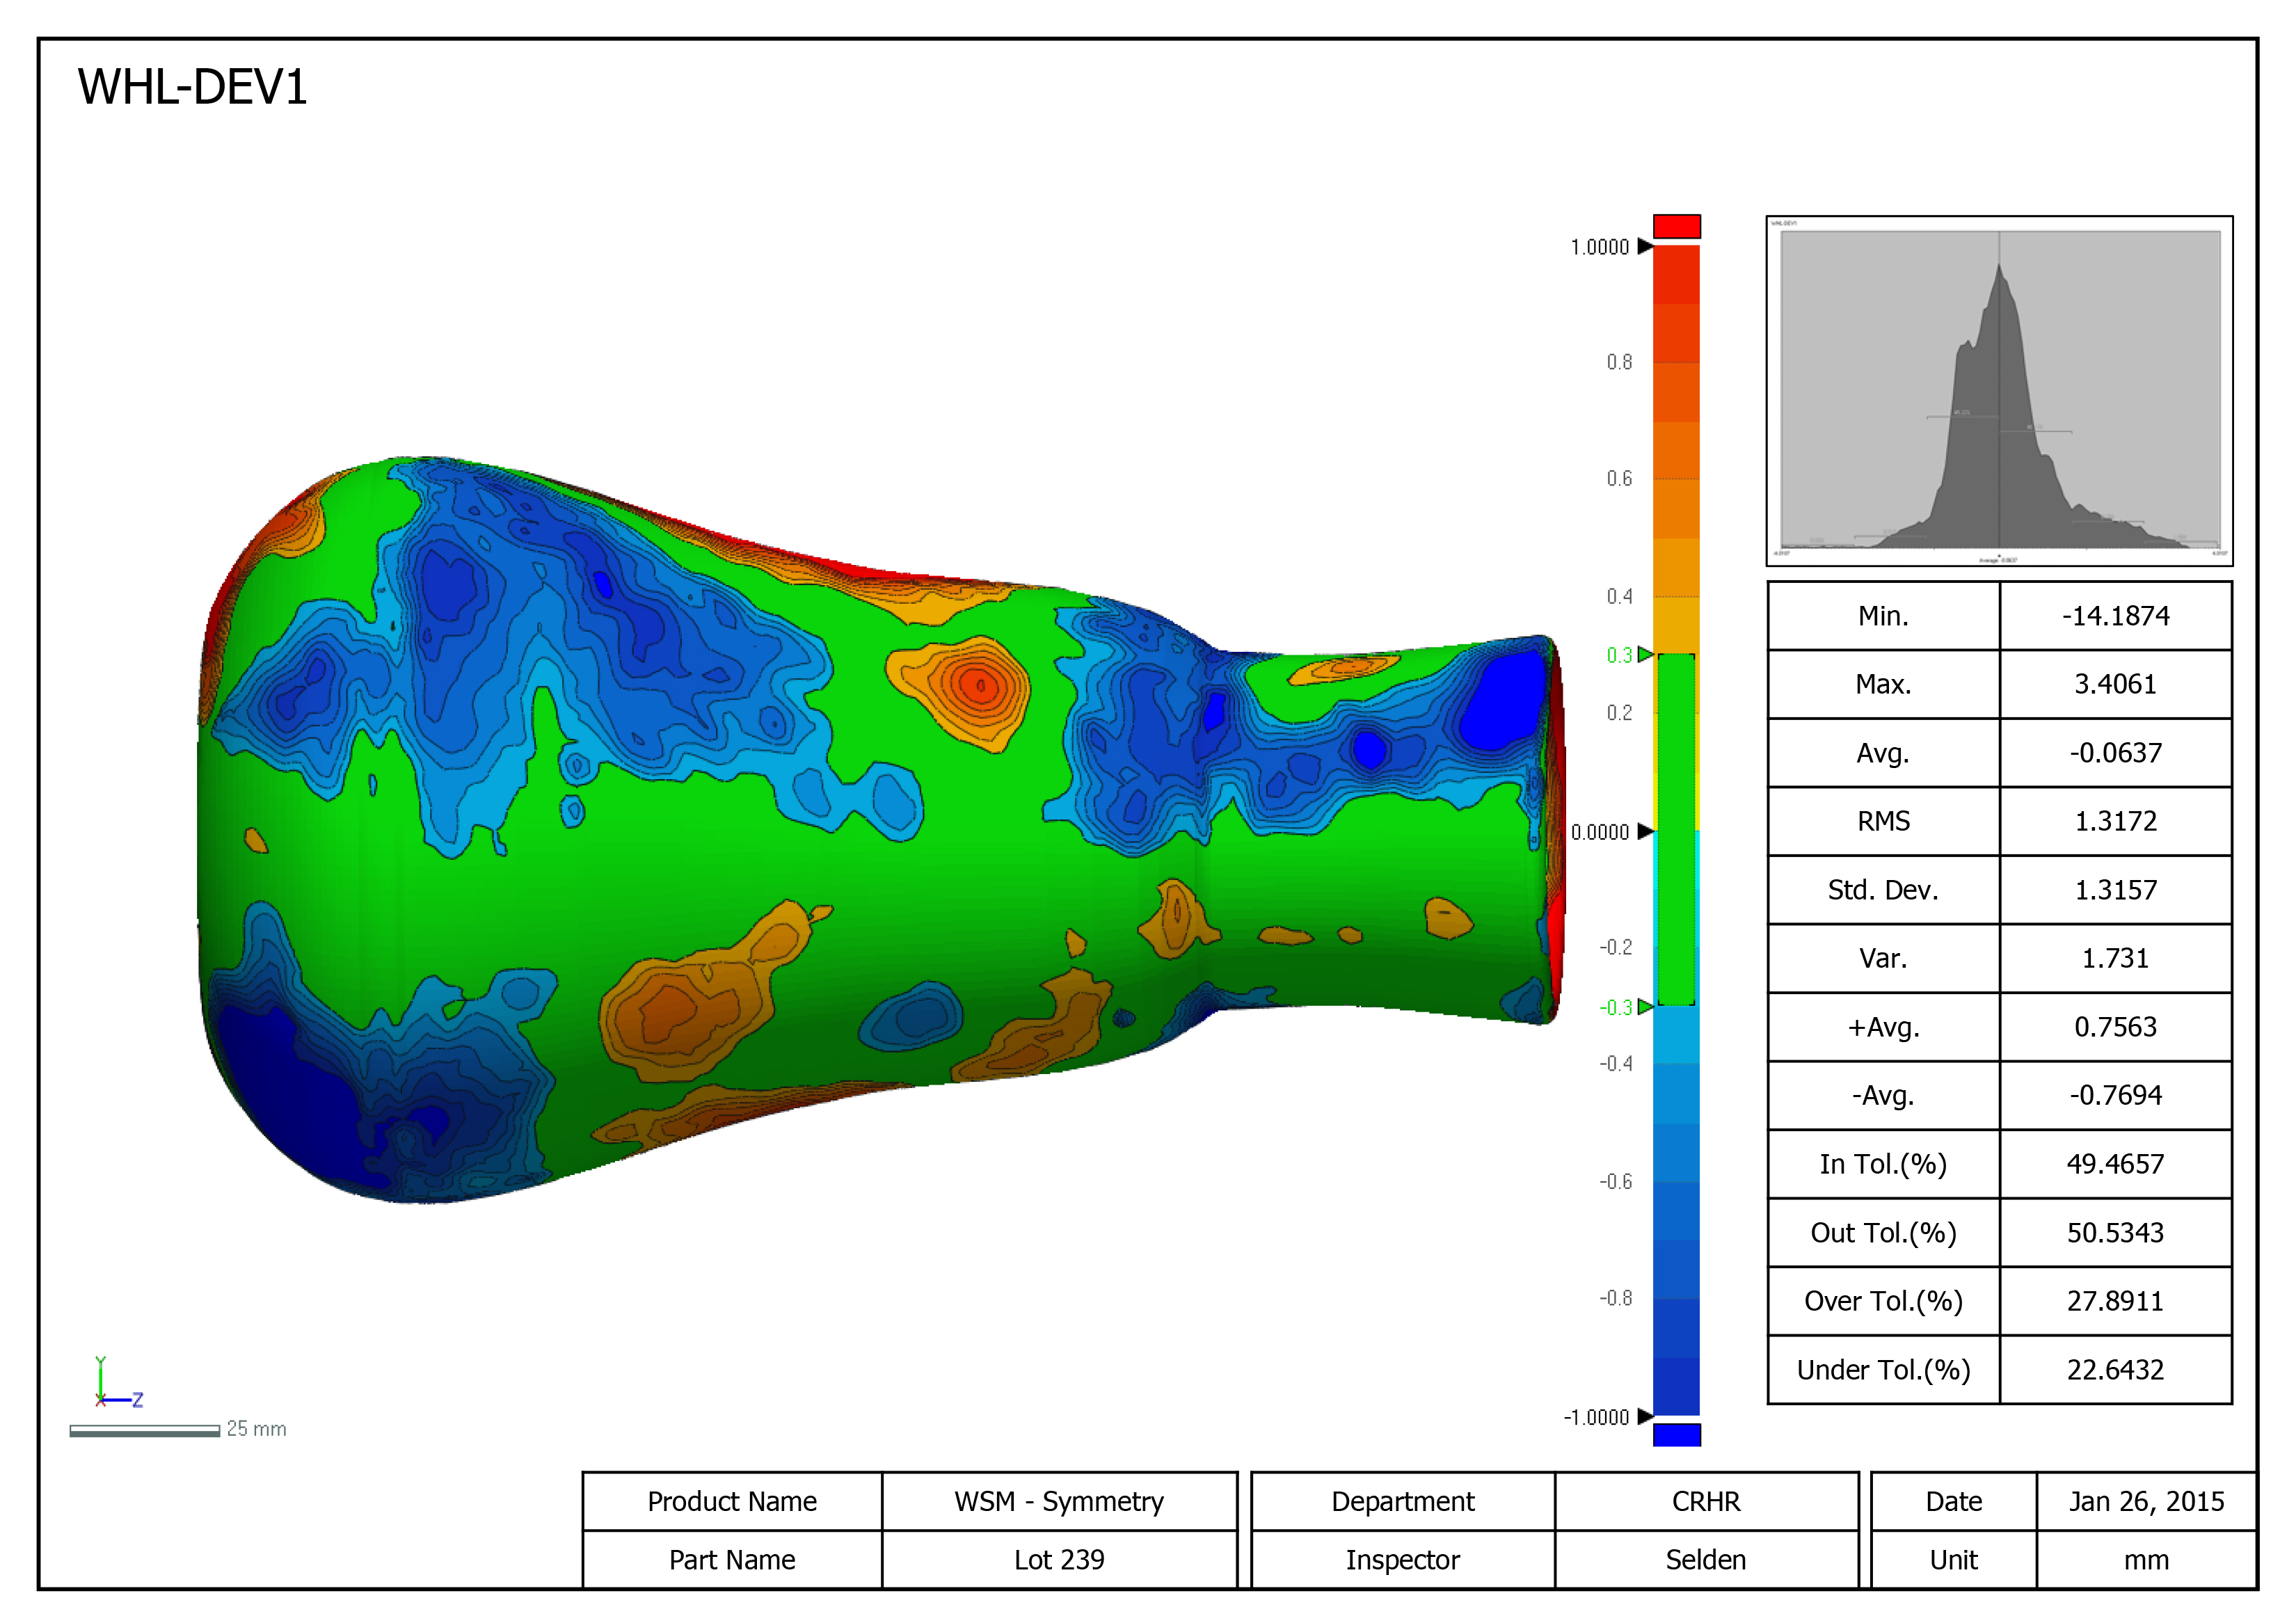
\includegraphics[width=\linewidth]{Selden-2017-Figure3}
\caption{Deviation between rotationally-symmetrical (nominal) surface and 3D scan data for Lot 239 from the Washington Square Mound site.}
\label{fig:Figure 5}
\end{figure}

The surface and the mesh were then imported to Geomagic Control X (inspection software), where deviations between the mesh and the symmetrical surface could be calculated for the whole vessel (Figure ~\ref{fig:Figure 5}), and the individual splines used in the analysis of geometric morphometrics (Figure ~\ref{fig:Figure 6}). Further, it is possible to export the landmark and adaptive sliding semilandmark points used in the geometric morphometric analysis to identify their deviation from the rotationally-symmetrical surface.

\begin{figure}[ht]\centering
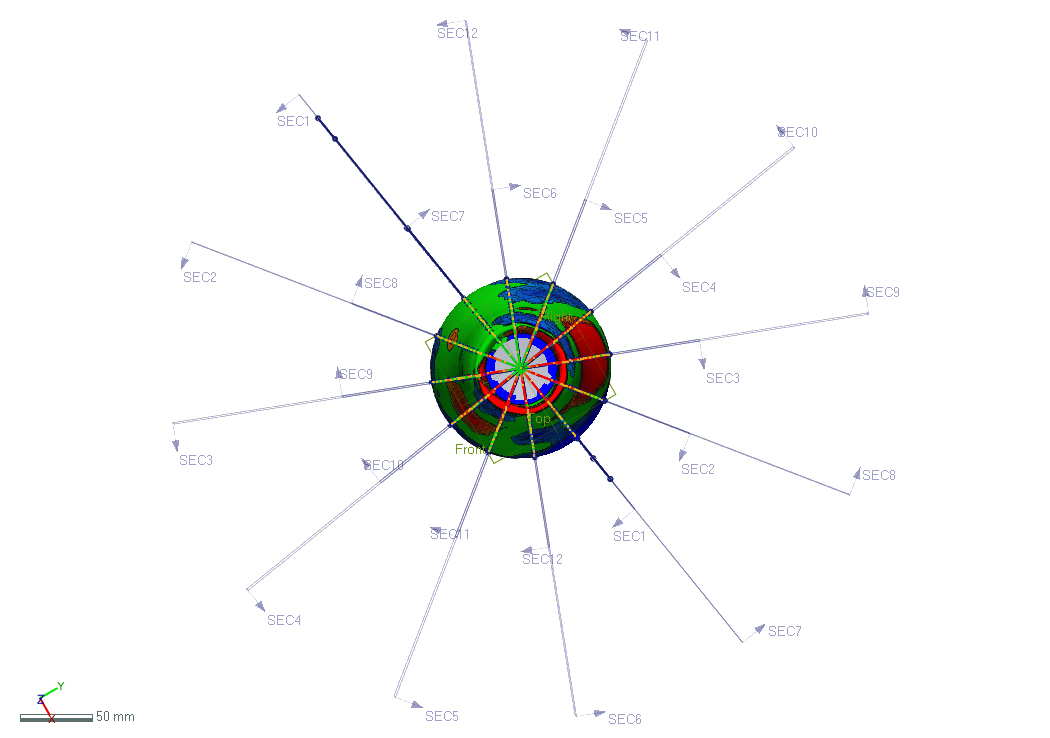
\includegraphics[width=\linewidth]{SS_2015_Figure_4}
\caption{Vessels can be sectioned, where the deviations for a specific spline can be extracted for a more in-depth analysis.}
\label{fig:Figure 6}
\end{figure}

\section{Results}

Results of the asymmetry analysis (Figures ~\ref{fig:Figure 5} and ~\ref{fig:Figure 7}) identified a percentage of each vessel that was within the specified (0.3mm) tolerance. These results were used in a comparison of fine wares and utility wares, and a comparison of vessel forms. The vessel in Figure ~\ref{fig:Figure 5} demonstrates the dynamic discrepancy that can be seen between the mesh and the rotationally-symmetrical surface. This is noteworthy for several reasons; principally to illustrate that the many vessel profiles found in the archaeological literature may be accurate, but are representative of only a very small part of the whole (note the small green area from the base to the rim in Figure ~\ref{fig:Figure 5}). The dynamic nature of ceramic artifacts is known to analysts, but our capacity to demonstrate these dynamics has to this point been limited by our systematics. 

\begin{figure}[ht]\centering
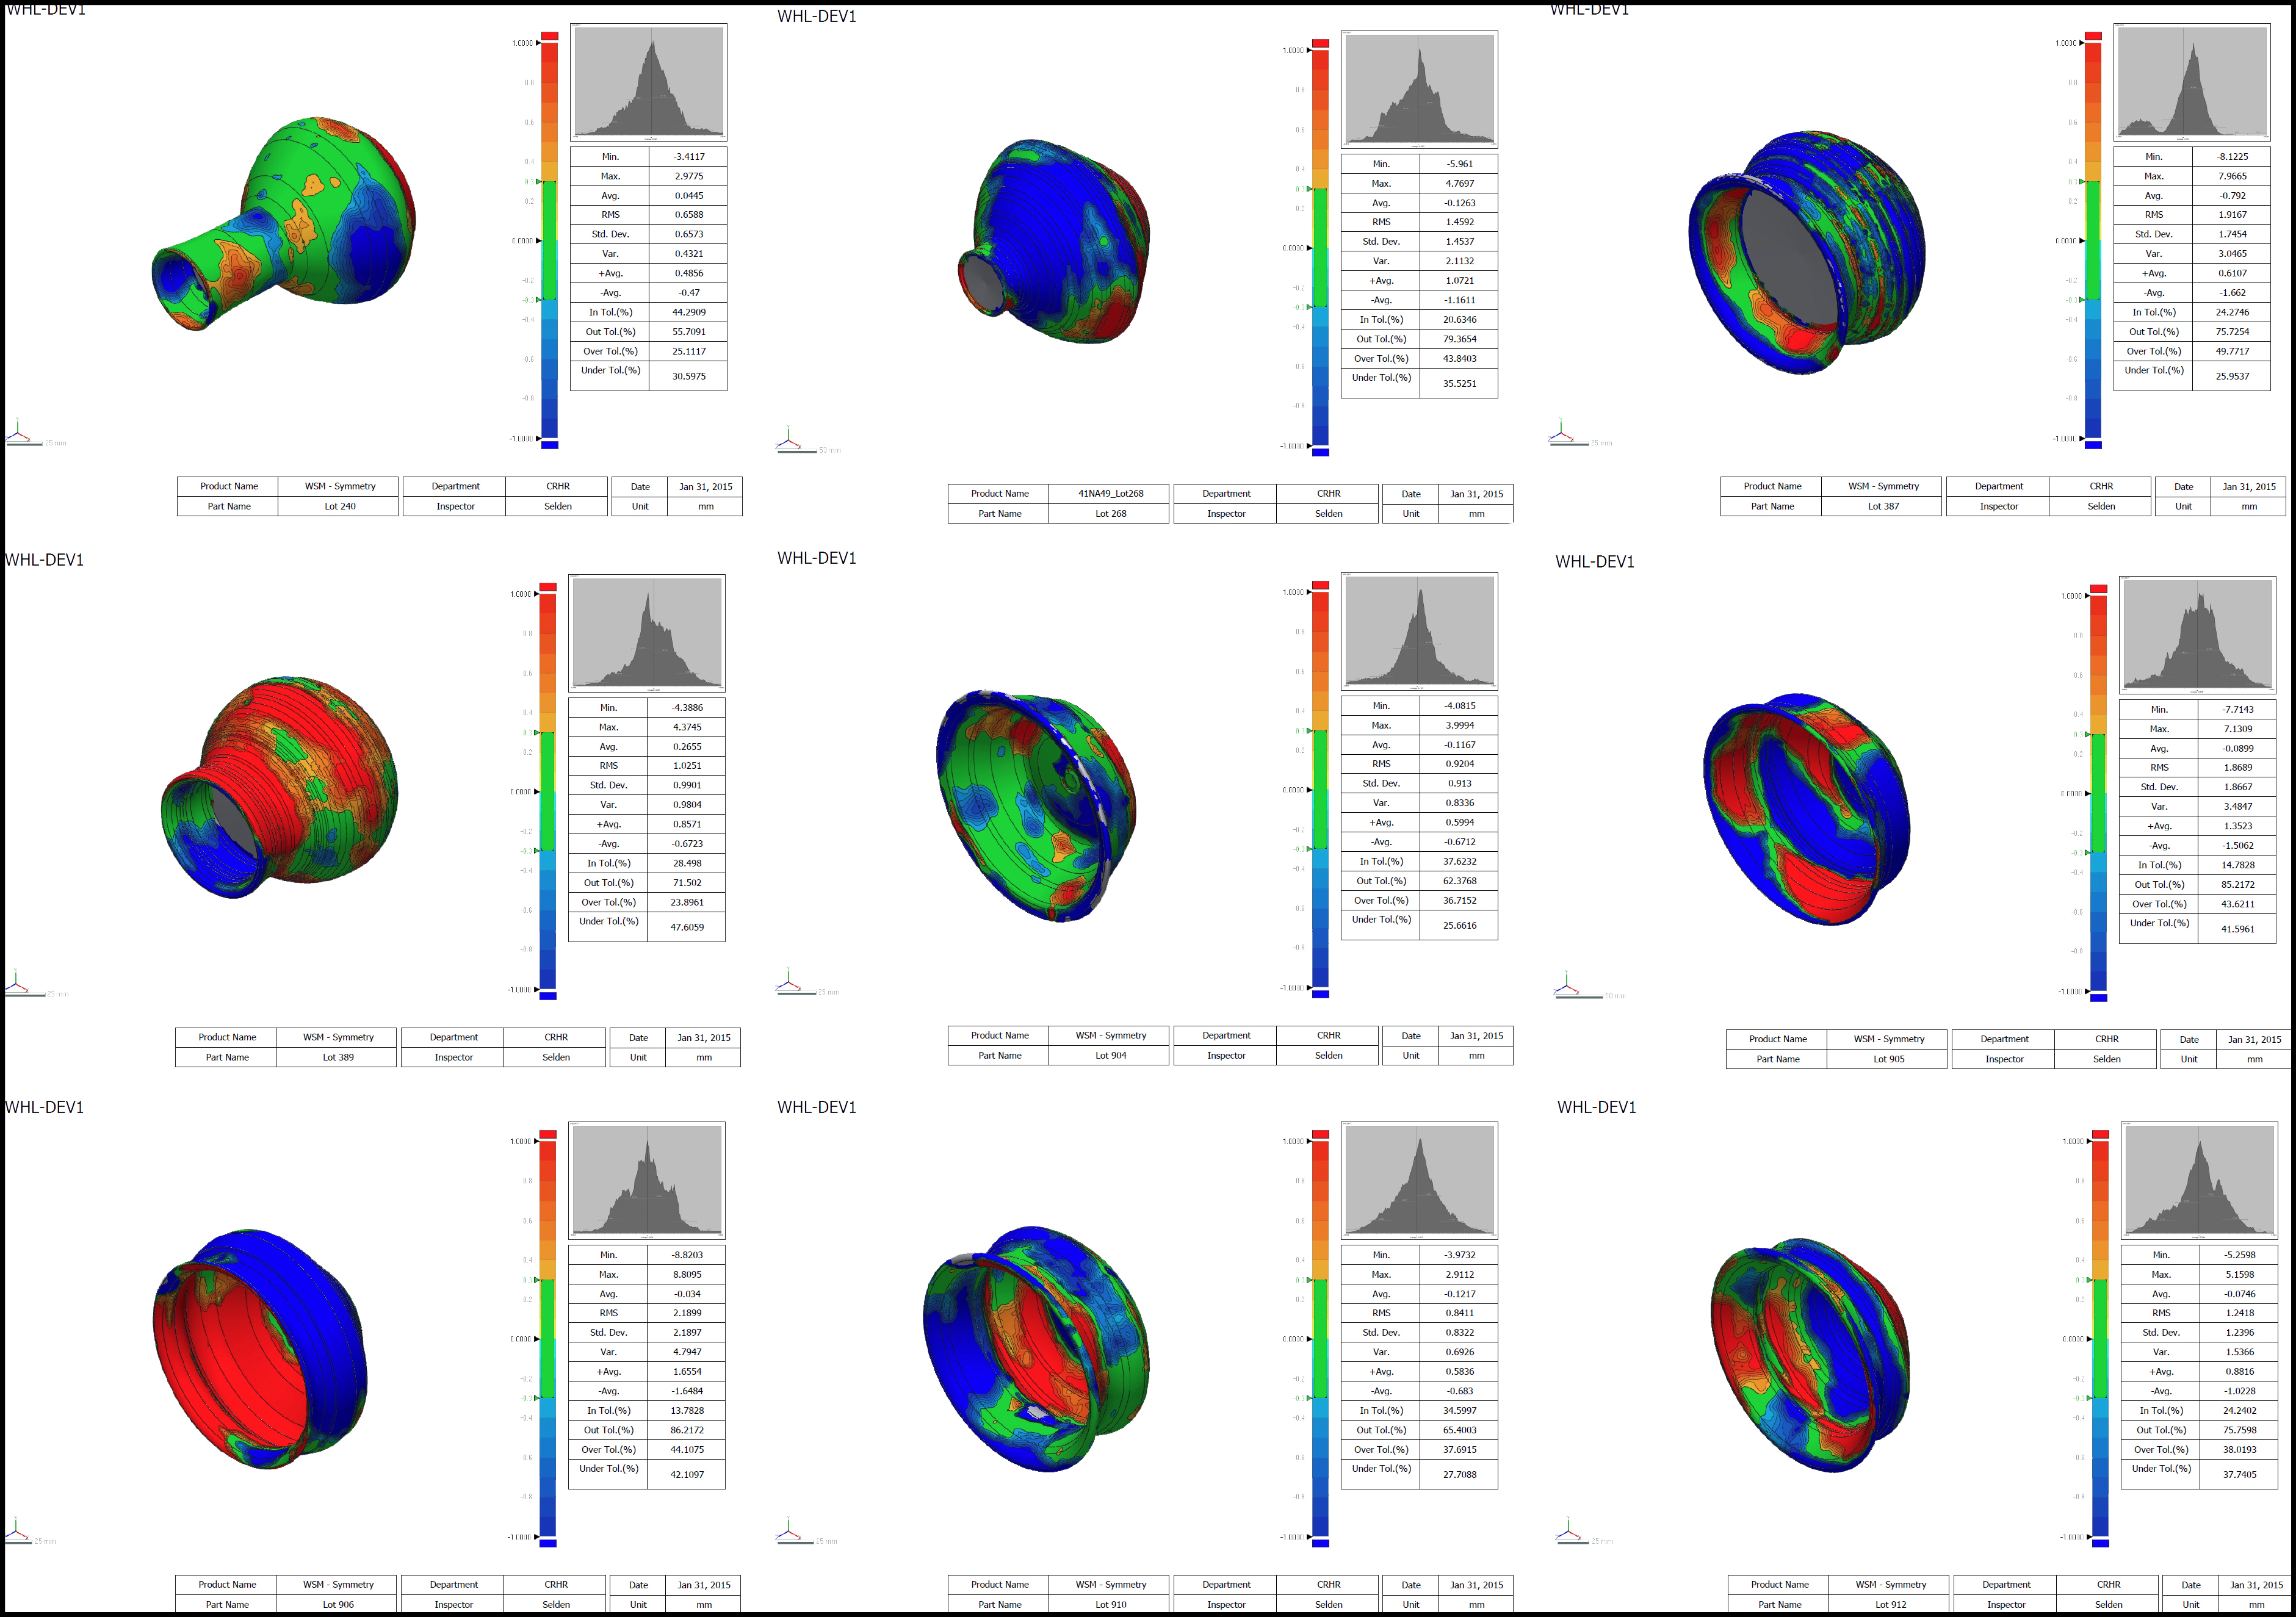
\includegraphics[width=\linewidth]{SS_2015_Figure_5}
\caption{Results of the asymmetry analysis.}
\label{fig:Figure 7}
\end{figure}

Of the two archaeological features where these vessels were recovered, only Feature 31 (F31) included both fine and utility wares. For that reason, a comparison of the fine (engraved) and utility (punctated, brushed and incised) wares was only conducted for F31, which yielded a substantial deviation between the two (Figure ~\ref{fig:Figure 8}a). Further, once segregated by vessel form (bottles, jars and an olla for F31), all were found to be within a range unique to each vessel shape (Figure ~\ref{fig:Figure 8}b). 

\begin{figure}[ht]\centering
\includegraphics[width=\linewidth]{S_2016_Fig9}
\caption{Comparison of (a) fine and utility wares from F31, and (b) bottles, jars and olla from F31.}
\label{fig:Figure 8}
\end{figure}

\subsection{Future Directions}

The development of the landmark configuration used in the geometric morphometric analysis can be seen as the first step in a hierarchically-nested method of inquiry. Additional modifications to the configuration of landmarks and sliding adaptive semilandmarks will be based upon specific research questions for the ceramic vessel assemblage(s) under study, and will likely consist of splitting each of the splines at well-defined junctions (base/body, body/rim, etc.) where the evolution of specific elements of ceramic vessel design (bottle necks, body, rim, etc) might be further explored. 

In an effort to better understand how studies of asymmetry employing geometric morphometrics articulate with one another, a citation network was generated that includes publication and citation data harvested from Scopus (Figure ~\ref{fig:FigureNetwork}). Once built, the network allows for the identification of methods and case studies that are most relevant to this research design, while also aiding in the identification of useful works that may not have been captured by the initial literature review. 

\begin{figure}[ht]\centering
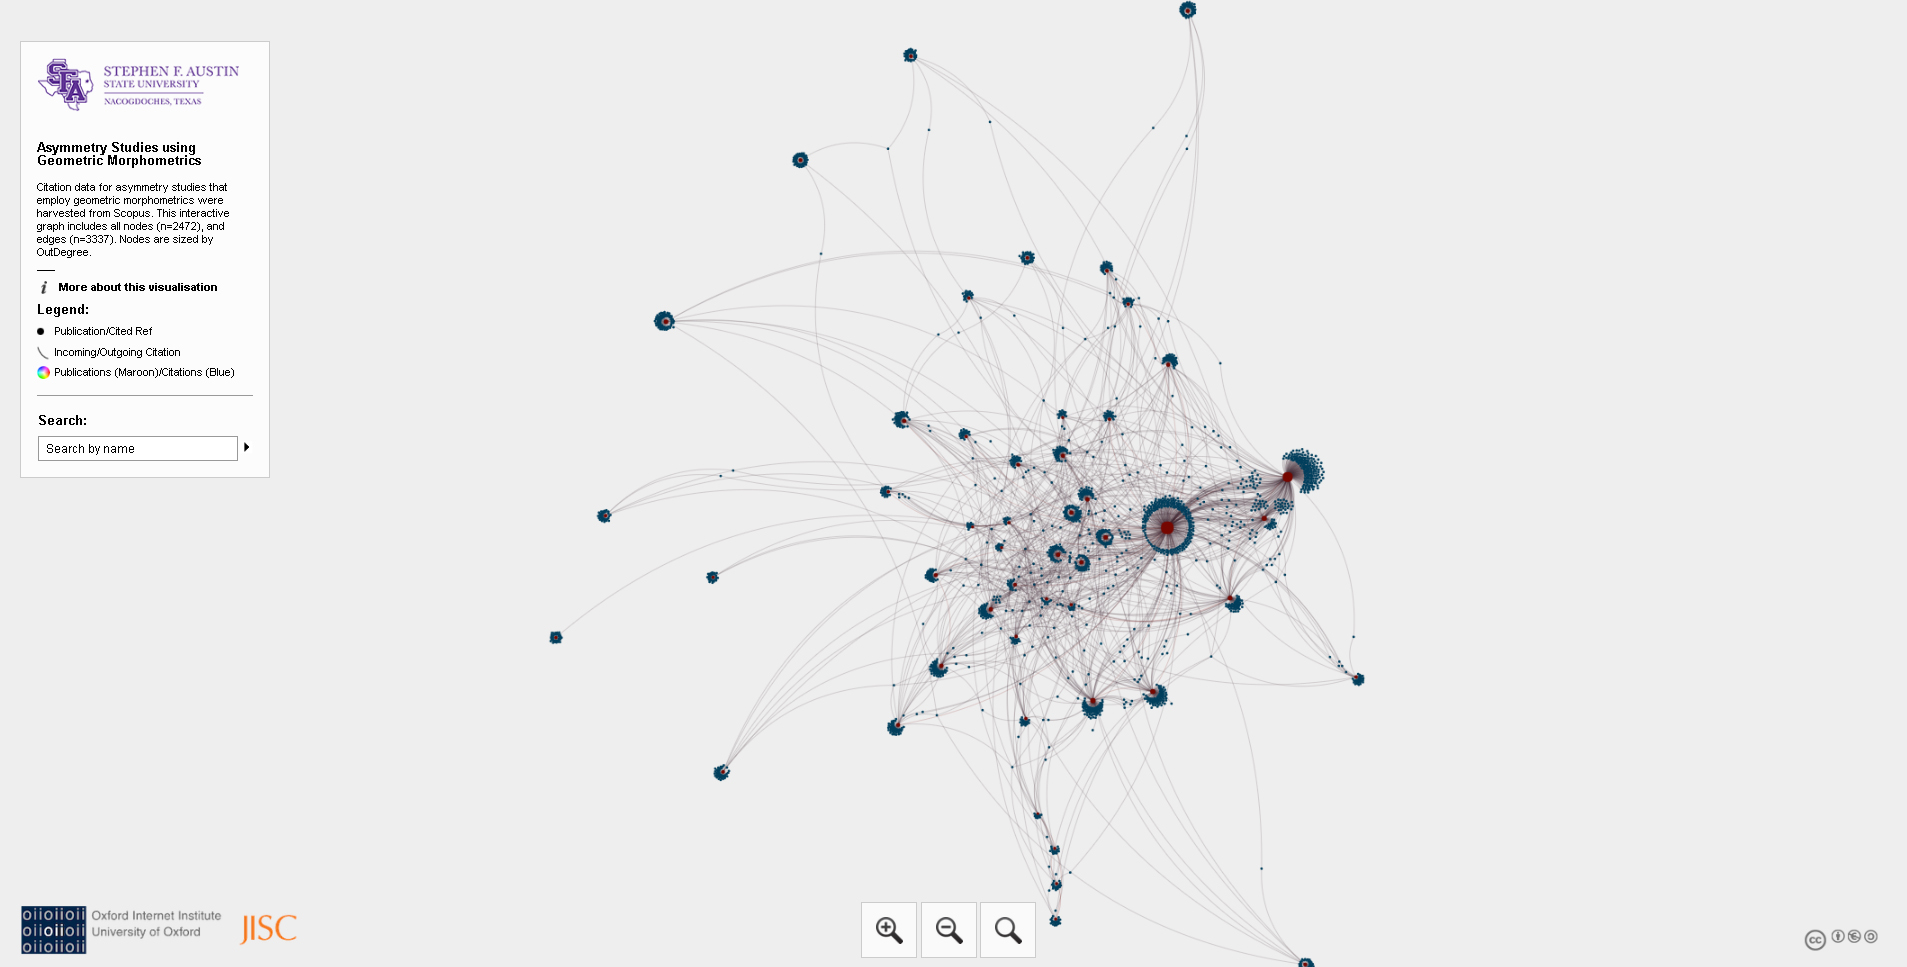
\includegraphics[width=\linewidth]{FigNet1}
\caption{Interactive citation network of publications and cited works for asymmetry studies that employ geometric morphometrics. Data harvested from Scopus. This interactive graph includes all nodes in the network (n=2472), and all edges (n=3337). Nodes are sized by OutDegree. View and interact with this network \href{http://crhr-archive.sfasu.edu/AsymmetryIntFig1/}{here}.}
\label{fig:FigureNetwork}
\end{figure}

The splines, landmarks and semi-landmark configurations developed for the geometric morphometric study can also be used to explore the variation that occurs in directional and--possibly--fluctuating asymmetry \citep{Klingenberg:3} (Figure ~\ref{fig:Figure 8}); both of which are becoming more regularly incorporated in analyses of geometric morphometrics (see Figure ~\ref{fig:FigureNetwork}). It is possible that measures of directional and fluctuating asymmetry will be found to b be more readily incorporated in the analysis than measures of rotational asymmetry.

\begin{figure}[ht]\centering
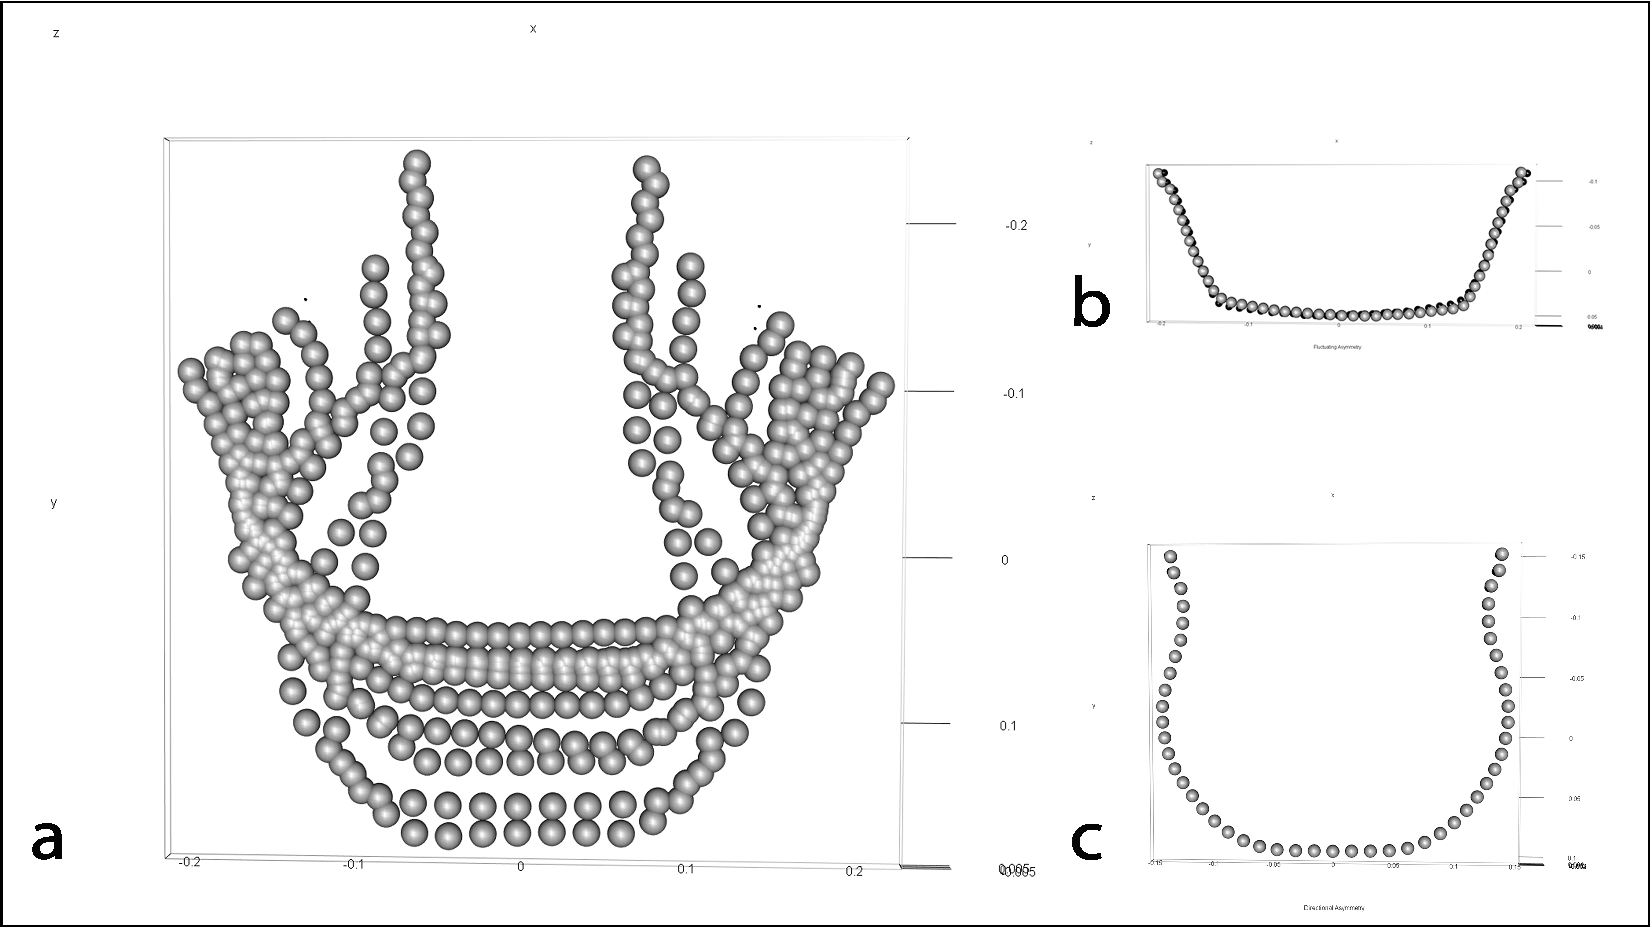
\includegraphics[width=\linewidth]{SS_2015_FigureX}
\caption{Results of a) generalized Procrustes analysis, b) analysis of fluctuating asymmetry and c) analysis of directional asymmetry.}
\label{fig:Figure 8}
\end{figure}

\section{Discussion}

The extent to which these data might inform upon variations in Caddo manufacturing practices for a specific temporal span is currently unknown. Testing these results by including samples from additional sites and temporal components should help to clarify whether--and to what extent--these data might inform upon possible shifts within, and between, groups of makers that employed differing methods of manufacture that may have resulted in variable degrees of conformity to rotational symmetry. As the resolution of the temporal dynamics in the East Texas region of the ancestral Caddo territory continues to be synthesized \citep{Selden:6}, refined \citep{Selden:4} and further explored \citep{Selden:5}, the fluid and dynamic nature of the Caddo ceramic economy should similarly increase in resolution. That same line of questioning may also inform upon whether those vessel shapes that transcend specific temporal boundaries have a consistent measure of rotational symmetry.

In a recent study of 3D geometric morphometrics for Caddo ceramics \citep{Selden:2}, several potentially meaningful results were achieved. Among these was the successful discrimination between the vessel shapes (bowls, jars, etc.). Within that study, subdivisions of vessel shape were identified, which were subsequently found to correlate with various qualitative attributes. This led to the discovery that variations in bowls, jars, and bottle categories may--in some way--be related to offerings, and that angular carinated bowls were associated with the use of red pigment in engraved designs, while globular carinated bowls were associated with the use of white pigment in engraved designs \citep{Selden:2}. Additionally, the carinated bowls were the only vessel shape to be included in all burials \citep{Selden:2}. The extent to which analyses of geometric morphometrics and rotational asymmetry will complement one another is yet unknown; however, there is precedent in the biological sciences  \cite{Savriama:1, Savriama:2}, and the functions needed to generate similar analyses for fluctuating and directional asymmetry are included in many of the current software packages used to study geometric morphometrics.

These preliminary results point toward the potential for significant theoretical gains; particularly for discussions related to the ceramic economy, where value is ascribed. While the notion of the attractiveness in a symmetrical shape is not a novel idea, the systematics associated with quantifying asymmetry for ceramics have long escaped us. The approach posited here allows for the collection of those metrics in three-dimensions. Importantly, the analysis also demonstrates that the many profiles contained in the published literature may be very useful for ongoing discussions of ceramic shape \cite{Wilczek:1}, but these 2D representations should only be revolved to illustrate vessel shape; and not to analyze it.

\section{Acknowledgments}

Many thanks to Dr. Michael J. Shott for the stimulating discussion that served as the catalyst that led to the development of this approach. I also thank Dr. Timothy K. Perttula and Dr. John P. Hart for their thoughtful comments on an earlier draft, and the MORPHMET community for feedback and constructive criticisms on an earlier iteration of the citation network.

\section{References Cited}

\bibliographystyle{model1-num-names}
\bibliography{SymMorph.bib}

\end{document}

%%
%% End of file